\documentclass[11pt]{article}
\usepackage{../cs70,latexsym,epsf}
\lecture{18}
\def\title{Lecture \the\lecturenumber}

%%% Alistair's Macros
\makeatletter
\def\eqalign#1{\,\vcenter{\openup\jot\m@th
  \ialign{\strut\hfil${##}$&${{}##}$\hfil
      \crcr#1\crcr}}\,}
\def\eqalignno#1{\displ@y \tabskip\@centering
  \halign to\displaywidth{\hfil${##}$\tabskip\z@skip
    &${{}##}$\hfil\tabskip\@centering
    &\llap{$##$}\tabskip\z@skip\crcr
    #1\crcr}}
\makeatother
\def\third{{\textstyle{1\over 3}}}
\def\half{{\textstyle{1\over 2}}}
\def\quarter{{\textstyle{1\over 4}}}
\def\ul#1{\underline{#1}}
\def\VarOmega{\mathchar"10A }
\def\varOmega{\mathchar"10A }
\newenvironment{proposition}{\par\global\advance\theoremnumber by 1
{\bf Proposition \the\lecturenumber.\the\theoremnumber}:
\begingroup\em}%
{\endgroup}
\def\ignore#1{}
\def\Ex#1{{\rm E}(#1)}
\def\Var#1{{\rm Var}(#1)}
\def\Aset{{\cal A}}

\newcounter{thm}
\addtocounter{thm}{\the\lecturenumber}
\newtheorem{corollary}{Corollary}[thm]
\newtheorem{theorem}{Theorem}[thm]
\newtheorem{definition}{Definition}[thm]

\begin{document}
\maketitle

\section*{Chebyshev's Inequality}

\subsubsection*{Problem: Estimating the Bias of a Coin}

Suppose we have a biased coin, but we don't know what the bias is. To estimate the bias, we
toss the coin $n$ times and count how many Heads we observe. 
Then our estimate of the bias is given by $\hat p = \frac{1}{n} S_n$, where $S_n$
is the number of Heads in the $n$ tosses. Is this a good estimate? Let $p$ denote the
true bias of the coin, which is unknown to us. Since $\Ex{S_n} = np$, we see that
the estimator $\hat p$ has the correct expected value: $\Ex{\hat p} = \frac{1}{n} \Ex{S_n} = p$.
This means when $n$ is sufficiently large, we can expect $\hat p$ to be very close to
$p$; this is a manifestation of the {\em Law of Large Numbers}, which we shall see at the end
of this note.

How large should $n$ be to guarantee that our estimate $\hat p$ is within
an error $\epsilon$ of the true bias $p$, i.e., $|\hat p - p| \le \epsilon$? 
The answer is that we can never guarantee with absolute certainty that
$|\hat p - p| \le \epsilon$. This is because $S_n$ is a random variable that can
take any integer values between $0$ and $n$, and thus $\hat p = \frac{1}{n} S_n$ 
is also a random variable that can take any values between $0$ and $1$. So regardless of the value of
the true bias $p \in (0,1)$, it is possible that in our experiment of $n$ coin tosses
we observe $n$ Heads (this happens with probability $p^n$), in which case $S_n = n$ and $\hat p = 1$.
Similarly, it is also possible that all $n$ coin tosses come up Tails (this happens with probability $(1-p)^n$),
in which case $S_n = 0$ and $\hat p = 0$. 

So instead of requiring that $|\hat p - p| \le \epsilon$ with absolute certainty, we relax our requirement
and only demand that $|\hat p - p| \le \epsilon$ with {\em confidence} $\delta$, namely,
$\Pr[|\hat p - p| \le \epsilon] \ge 1-\delta$. This means there is a small probability $\delta$ that we make
an error of more than $\epsilon$,  but with high probability (at least $1-\delta$) our estimate is very close
to $p$. Now we can state our result: to guarantee that $\Pr[|\hat p - p| \le \epsilon] \ge 1-\delta$, it suffices
to toss the coin $n$ times where $$n \ge \frac{1}{4\epsilon^2 \delta}.$$

To prove such a result we use the tool called {\em Chebyshev's Inequality}, which 
provides a quantitative bound on how far away a random variable is from its expected value.


\subsection*{Markov's Inequality}

Before going to Chebyshev's inequality, we first state the following 
simpler bound, which applies only to {\it non-negative\/} random variables
(i.e., r.v.'s which take only values $\ge 0$).

\begin{theorem}[{\bf Markov's Inequality}] For a {\em non-negative}
random variable~$X$ with expectation $\Ex{X}=\mu$, and any $\alpha>0$, $$
   \Pr[X\ge\alpha]\le{{\Ex{X}}\over\alpha}.  $$
\end{theorem}

\begin{proof} From the definition of expectation, we have $$
\eqalign{\Ex{X}&=\sum_a a\times\Pr[X=a]\cr
               &\ge \sum_{a\ge\alpha} a\times\Pr[X=a]\cr
               &\ge \alpha\sum_{a\ge\alpha} \Pr[X=a]\cr
               &=\alpha\Pr[X\ge\alpha].\cr} $$
 Rearranging the inequality gives us the desired result. 
The crucial step here is the second line, where we have used the
fact that $X$ takes on only non-negative values. (Why is this step
not valid otherwise?)
\end{proof}

There is an intuitive way of understanding Markov's inequality through an
analogy of a seesaw.  Imagine that the distribution of a non-negative random variable $X$
is resting on a fulcrum, $\mu = \Ex{X}$.  We are trying to find an upper bound on the percentage
of the distribution which lies beyond $k \mu$, i.e., $\Pr[X \ge k \mu]$.  In other words, we seek
to add as much weight $m_2$ as possible on the seesaw at $k \mu$ while minimizing the effect it has
on the seesaw's balance.  This weight will represent the upper bound we are searching for.  To minimize
the weight's effect, we must imagine that the weight of the distribution which lies beyond $k \mu$ is
concentrated at exactly $k \mu$.  However, to keep things stable and maximize
the weight at $k \mu$, we must add another weight $m_1$ as far left to the fulcrum as we can so that $m_2$
is  as large as it can be.  The farthest we can go to the left is $0$, since $X$ is assumed to be non-negative.
Moreover, the two weights $m_1$ and $m_2$ must add up to $1$, since they represent the area under the
distribution curve:

\begin{figure}[h]
\centering
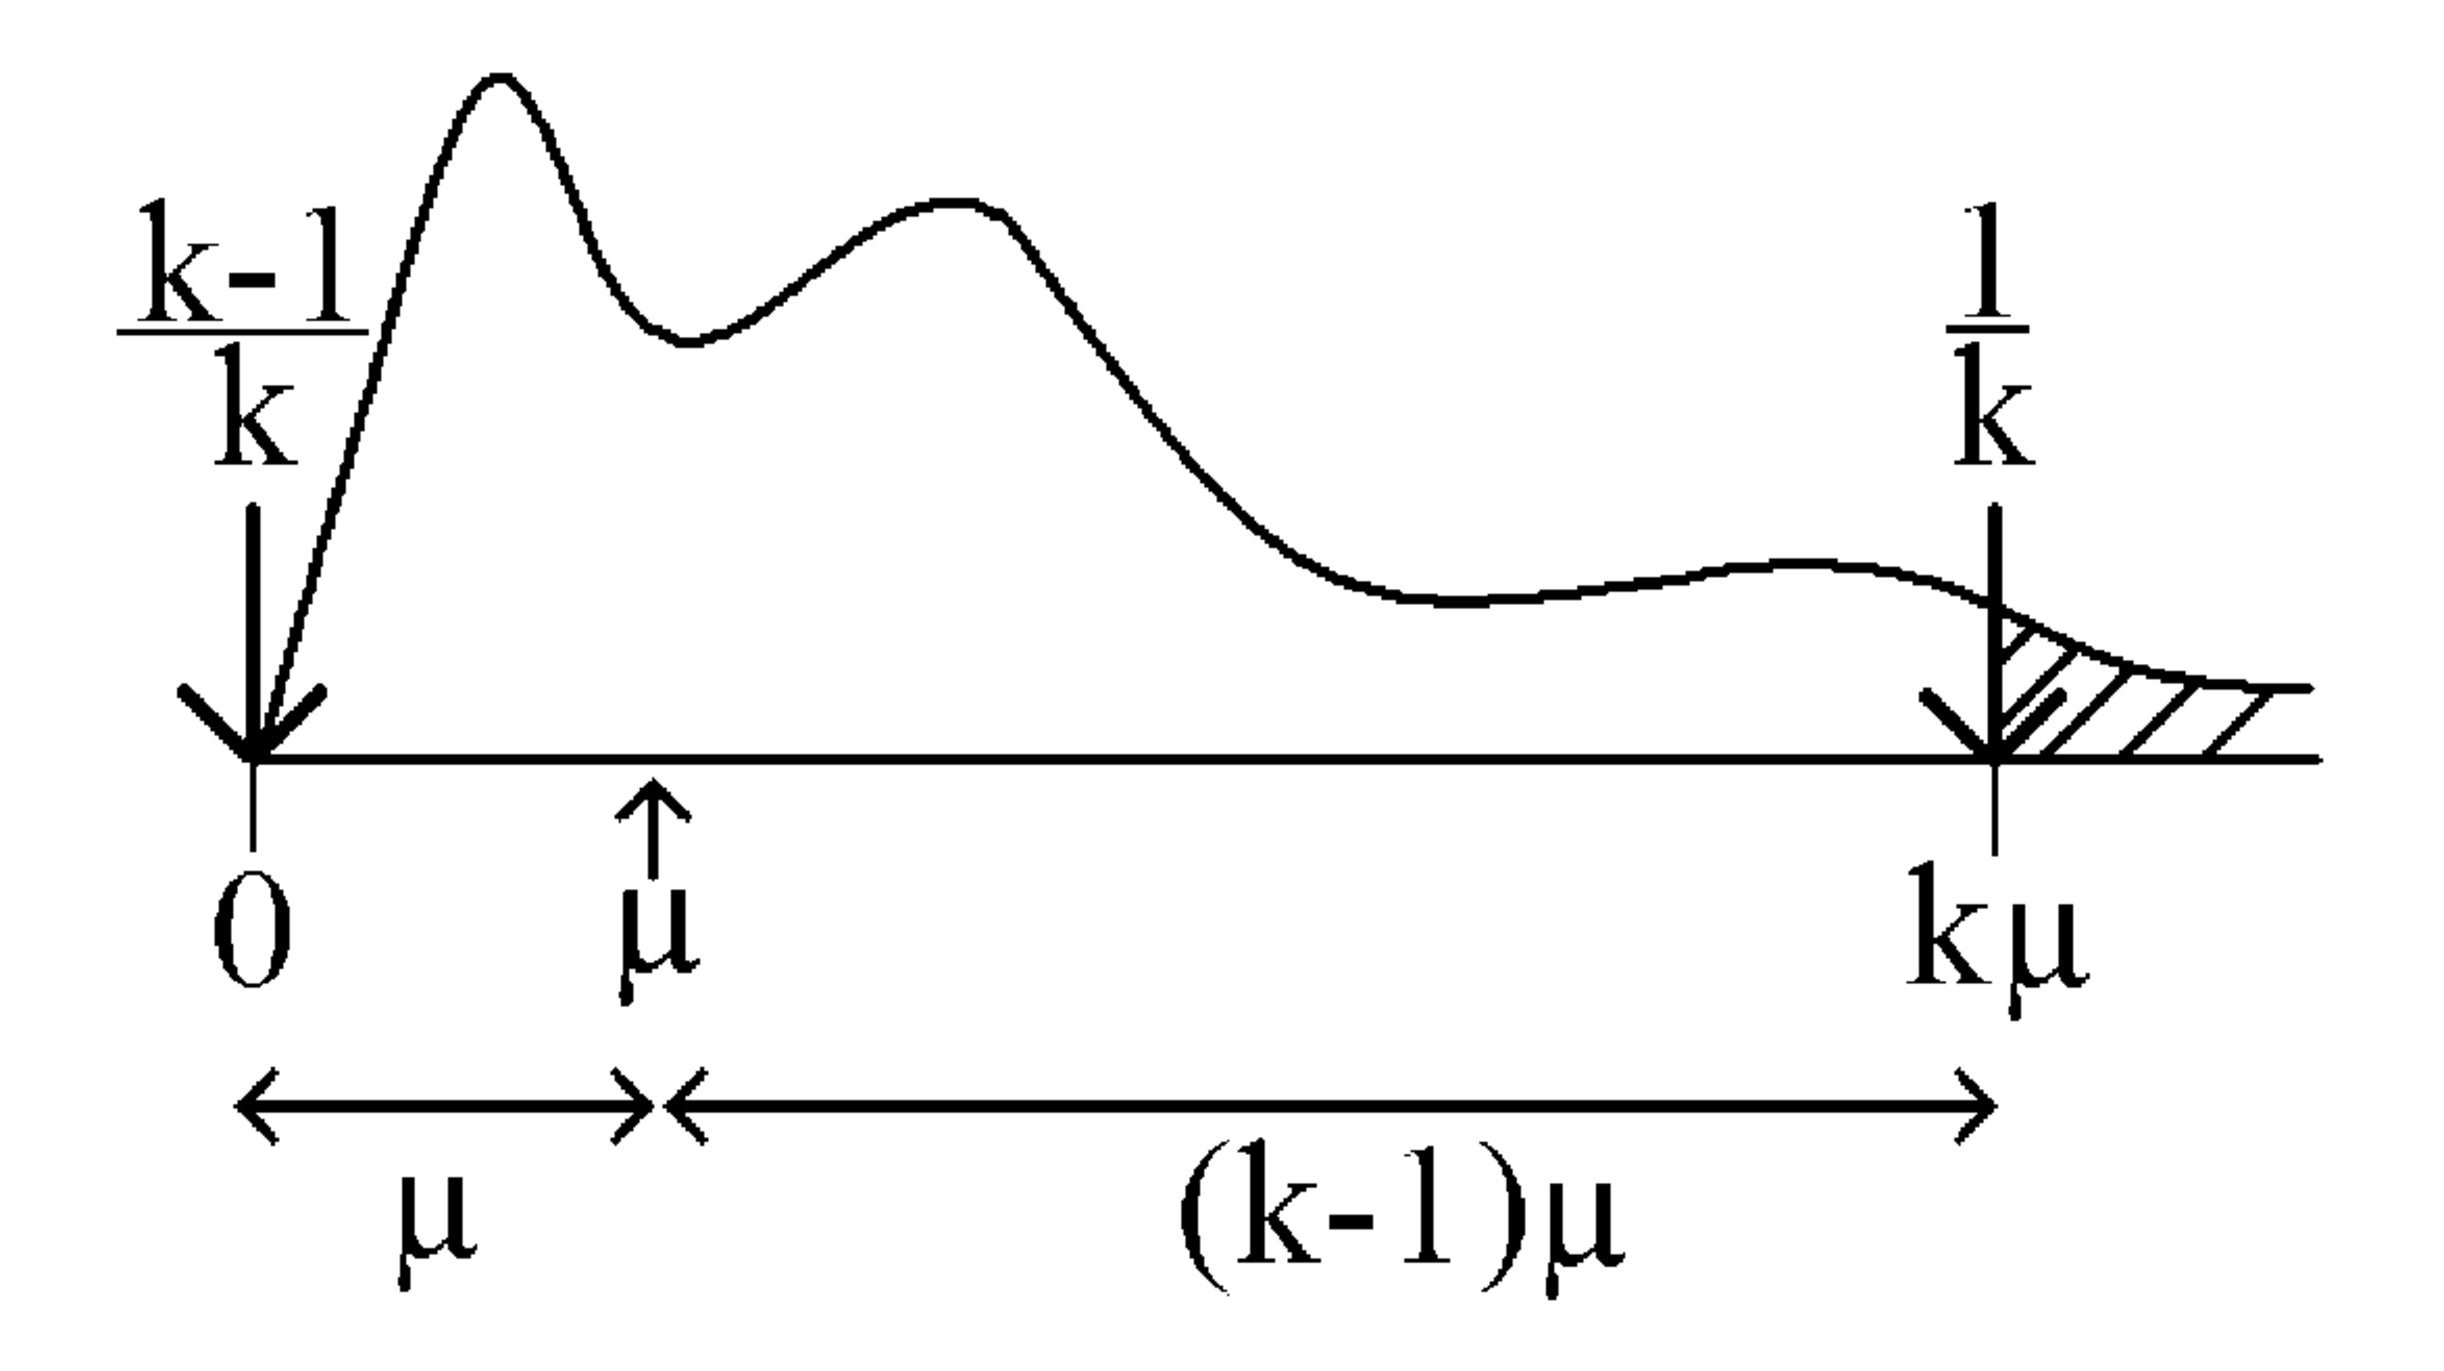
\includegraphics[scale=.24]{seasaw}
\caption{Markov's inequality interpreted as balancing a seesaw.}
\label{fig:seasaw}
\end{figure}

Since the lever arms are in the ratio $k-1$ to $1$, a unit weight at $k \mu$ balances $k-1$ units of weight
at $0$. So the weights should be $\frac{k-1}{k}$ at $0$ and $\frac{1}{k}$ at $k\mu$, which is exactly 
Markov's bound with $\alpha = k\mu$. 




\subsection*{Chebyshev's Inequality}

We have seen that, intuitively, the variance (or, more correctly
the standard deviation) is a measure of
``spread,'' or deviation from the mean.  We can now make
this intuition quantitatively precise:

\begin{theorem}[{\bf Chebyshev's Inequality}] For a random variable~$X$
with expectation $\Ex{X}=\mu$, and for any $\alpha>0$,  $$
   \Pr[|X-\mu|\ge\alpha] \le {{\Var{X}}\over{\alpha^2}}.  $$
\end{theorem}
\begin{proof}
Define the random variable $Y=(X-\mu)^2$.
Note that $\Ex{Y}=\Ex{(X-\mu)^2}=\Var{X}$.  Also, notice that
the event that we are interested in, $|X-\mu| \ge \alpha$, is
exactly the same as the event $Y = (X-\mu)^2 \ge \alpha^2$.
Therefore, $\Pr[|X-\mu| \ge \alpha] = \Pr[Y \ge \alpha^2]$.
Moreover, $Y$ is obviously non-negative, so we can apply Markov's inequality
to it to get $$
  \Pr[Y\ge\alpha^2] \le {{\Ex{Y}}\over{\alpha^2}} = {{\Var{X}}\over{\alpha^2}}. $$
This completes the proof.
\end{proof}

Let's pause to consider what Chebyshev's inequality says.
It tells us that the probability of any given deviation,
$\alpha$, from the mean, either above it or below it (note the
absolute value sign), is at most ${{\Var{X}}\over{\alpha^2}}$.
As expected, this deviation probability will be small if the
variance is small.  An immediate corollary of Chebyshev's
inequality is the following:

\begin{corollary} For a random variable~$X$
with expectation $\Ex{X}=\mu$, and standard deviation
$\sigma=\sqrt{\Var{X}}$, $$
   \Pr[|X-\mu|\ge\beta\sigma] \le {1\over{\beta^2}}.  $$
\end{corollary}

\begin{proof} Plug $\alpha=\beta\sigma$ into Chebyshev's inequality.
\end{proof}

So, for example, we see that the probability of deviating from
the mean by more than (say) two standard deviations on either side
is at most~$1\over 4$.  In this sense, the standard deviation is
a good working definition of the ``width'' or ``spread'' of a distribution.

In some special cases it is 
possible to get tighter bounds on the probability of deviations from
the mean.  However, for general random variables Chebyshev's inequality
is essentially the only tool.  Its power derives from the fact that it can be
applied to {\it any\/} random variable. 



\subsection*{Example: Estimating the Bias of a Coin}

Let us go back to our motivating example of estimating the bias of a coin.
Recall that we have a coin of unknown bias $p$, and our estimate of $p$
is $\hat p = \frac{1}{n} S_n$ where $S_n$ is the number of Heads
in $n$ coin tosses.

As usual, we will find it helpful to write $S_n = X_1 + \cdots + X_n$,
where $X_i = 1$ is the $i$-th coin toss comes up Heads and $X_i = 0$
otherwise, and the random variables $X_1,\dots,X_n$ are mutually independent.
Then $\Ex{X_i} = \Pr[X_i = 1] = p$, so by linearity of expectation,
$$\Ex{\hat p} = \Ex{\textstyle{\frac{1}{n}} S_n} = \textstyle{\frac{1}{n}} \sum_{i=1}^n \Ex{X_i} = p.$$
What about the variance of $\hat p$? Note that
since the $X_i$'s are independent, the variance of $S_n = \sum_{i=1}^n X_i$ is equal to
the sum of the variances:
$$\Var{\hat p} = \Var{{\textstyle{\frac{1}{n}}} S_n} = \textstyle{\frac{1}{n^2}} \Var{S_n}
= \textstyle{\frac{1}{n^2}} \sum_{i=1}^n \Var{X_i} = \frac{\sigma^2}{n},$$
where we have written $\sigma^2$ for the variance of each of the $X_i$.

So we see that \ul{the variance of $\hat p$ decreases
linearly with~$n$}. This fact ensures that, as we take larger
and larger sample sizes~$n$, the probability that we deviate much
from the expectation~$p$ gets smaller and smaller.

Let's now use Chebyshev's inequality to figure out how large $n$ has
to be to ensure a specified accuracy in our estimate of the true bias $p$.
As we discussed in the beginning of this note, a natural way to measure this is for
us to specify two parameters, $\epsilon$ and~$\delta$, both in the
range $(0,1)$. The parameter $\epsilon$ controls the {\it error\/}
we are prepared to tolerate in our estimate, and~$\delta$ controls
the {\it confidence\/} we want to have in our estimate.

Applying Chebyshev's inequality, we have 
$$
   \Pr[|\hat p-p|\ge \epsilon] \le \frac{\Var{\hat p}}{\epsilon^2}
                              = \frac{\sigma^2}{n\epsilon^2}.  $$
To make this less than the desired value~$\delta$, we need to set
\begin{equation}\label{eq2}
   n\ge {{\sigma^2}\over{\epsilon^2\delta}}.
\end{equation}
Now recall that $\sigma^2=\Var{X_i}$ is the variance of a single
sample~$X_i$.  So, since $X_i$ is an indicator random variable with $\Pr[X_i = 1] = p$, we have
$\sigma^2 = p(1-p)$, and inequality~(\ref{eq2}) becomes
\begin{equation}\label{eq3}
   n\ge {{p(1-p)}\over {\epsilon^2\delta}}.
\end{equation}
Since $p(1-p)$ is takes on its maximum value for $p=1/2$, we can conclude
that it is sufficient to choose $n$ such that:
\begin{equation}\label{eq3}
   n\ge {{1}\over {4\epsilon^2\delta}},
\end{equation}
as we claimed earlier.

For example, plugging in $\epsilon=0.1$ and $\delta=0.05$, we see that a sample
size of $n=500$ is sufficient to get an estimate $\hat p$ that is accurate to within an error
of $0.1$ with probability at least $95\%$.

As a concrete example, consider the problem of estimating the proportion $p$ of
Democrats in the US population, by taking a small random sample. We can model this
as the problem of estimating the bias of a coin above, where each coin toss corresponds
to a person that we select randomly from the entire population. Our calculation above shows that
to get an estimate $\hat p$ that is accurate to within an error of $0.1$ with probability at least
$95\%$, it suffices to sample $n = 500$ people. In particular, notice that the size of the sample
is independent of the total size of the  population! This is how polls can accurately estimate quantities
of interest for  a population of several hundred million while sampling only a very small number
of people.  



\subsection*{Estimating a general expectation}

What if we wanted to estimate something a little more complex than
the bias of a coin? For example, suppose we want to estimate the
average wealth of people in the US. We can model this as the problem
of estimating the expected value of an unknown probability distribution.
Then we can use exactly the same scheme as before, except that now we sample the random
variables $X_1,X_2,\dots,X_n$ independently from our unknown distribution.
Clearly $\Ex{X_i}=\mu$, the expected value that we are trying to
estimate. Our estimate of $\mu$ will be $\hat \mu={1\over n}\sum_{i=1}^n X_i$,
for a suitably chosen sample size~$n$.

Following the same calculation as before, we have
$\Ex{\hat \mu}=\mu$ and $\Var{\hat \mu}={{\sigma^2}\over n}$, where
$\sigma^2=\Var{X_i}$ is the variance of the~$X_i$. (Recall that the
only facts we used about the $X_i$ was that they were independent
and had the same distribution --- actually the same expectation and
variance would be enough: why?) This time, however, since we do not
have any a priori bound on the mean $\mu$, it makes more
sense to let $\epsilon$ be the relative error, i.e., we wish to find
an estimate $\hat \mu$ that is within an additive error of $\epsilon\mu$:
$$
   \Pr[|\hat \mu-\mu|\ge \epsilon\mu] \le \delta.  $$
Using equation~(\ref{eq2}), but substituting $\epsilon\mu$ in place of 
$\epsilon$, it is enough for the sample size~$n$ to
satisfy
\begin{equation}\label{eq4}
   n\ge {{\sigma^2}\over{\mu^2}}\times{1\over{\epsilon^2\delta}}.
\end{equation}
Here $\epsilon$ and~$\delta$ are the desired relative error and confidence
respectively.  Now of course we don't know the other two
quantities, $\mu$ and~$\sigma^2$, appearing in equation~(\ref{eq4}).
In practice, we would use a lower bound on $\mu$ and an upper bound
on~$\sigma^2$ (just as we used a lower bound on $p$ in the coin tossing
problem).  Plugging these bounds into equation~(\ref{eq4}) will
ensure that our sample size is large enough.

For example, in the average wealth problem we could probably safely
take $\mu$ to be at least (say) \$20k (probably more).  However, the
existence of very wealthy people such as Bill Gates means that we would need to
take a very high value for the variance~$\sigma^2$.  Indeed, if
there is at least one individual with wealth \$50~billion, then
assuming a relatively small value of~$\mu$ means that the variance
must be at least about ${{(50\times 10^9)^2}\over{250\times 10^6}} =
10^{13}$. 
There is really no way around this problem with simple uniform
sampling: the uneven distribution of wealth means that the variance
is inherently very large, and we will need a huge number of samples
before we are likely to find anybody who is immensely wealthy.  But
if we don't include such people in our sample, then our estimate
will be way too low.


\section*{The Law of Large Numbers}
The estimation method we used in the previous sections is based
on a principle that we accept as part of everyday life: namely, the
Law of Large Numbers (LLN).  This asserts that, if we observe some
random variable many times, and take the average of the
observations, then this average will converge to a {\it single
value}, which is of course the expectation of the random variable.
In other words, averaging tends to smooth out any large
fluctuations, and the more averaging we do the better the smoothing.

\begin{theorem}[{\bf Law of Large Numbers}]
Let $X_1,X_2,\ldots,X_n$ be i.i.d.\ random variables with common
expectation $\mu=\Ex{X_i}$.  Define $A_n={1\over n}\sum_{i=1}^n
X_i$. Then for any $\alpha>0$, we have $$
 \Pr\left[|A_n-\mu|\ge\alpha\right] \to 0 \qquad\hbox{\rm as $n\to\infty$}.$$
\end{theorem}

\begin{proof}
Let $\Var{X_i}=\sigma^2$ be the common variance of the r.v.'s; we
assume that $\sigma^2$ is finite.\footnote{If $\sigma^2$ is not
finite, the LLN still holds but the proof is much trickier.} With
this (relatively mild) assumption, the LLN is an immediate
consequence of Chebyshev's Inequality. For, as we have seen above,
$\Ex{A_n}=\mu$ and $\Var{A_n}=\frac{\sigma^2}{n}$, so by Chebyshev
we have $$
 \Pr\left[|A_n-\mu|\ge\alpha\right] \le \frac{\Var{A_n}}{\alpha^2} = \frac{\sigma^2}{n\alpha^2}  \to 0 \qquad\hbox{\rm as $n\to\infty$}.$$
This completes the proof.
\end{proof}

Notice that the LLN says that the probability of {\it any\/}
deviation~$\alpha$ from the mean, however small, tends to zero as
the number of observations~$n$ in our average tends to infinity.
Thus by taking $n$ large enough, we can make the probability of any
given deviation as small as we like.


\end{document}
